\chapter{Implementation}

\section{Level Set Algorithm}\label{levelsetalgorithm}

\subsection{Upwinding}\label{upwinding}
Equation \eqref{eq:levelsetequation}, the level set equation, needs to be discretized for both sequential and parallel computation. This is done using the \textit{up-wind} differencing scheme. The following explanation of \textit{upwinding} is from \cite{osher2003lsm}.

A first order accurate method for time discretization of equation \eqref{eq:levelsetequation}, is given by the forward Euler method, from \cite{osher2003lsm}:

\begin{equation}
\frac{\phi^{t+\Delta t}-\phi^t}{\Delta t} +F^{t}\cdot{\nabla{\phi^{t}}} = 0
\label{eq:euler1}
\end{equation}

where $\phi^{t}$ represents the current values of $\phi$ at time $t$, $F^{t}$ represents the velocity field at time $t$, and  $\nabla{\phi^{t}}$ represents the values of the gradient of $\phi$ at time $t$. When computing the gradient, a great deal of care must be taken with regards to the spatial derivatives of $\phi$. This is best exemplified by considering the expanded form of equation \eqref{eq:euler1}.

\begin{equation}
\frac{\phi^{t+\Delta t}-\phi^t}{\Delta t} +u^{t}\phi_x^t+v^{t}\phi_y^t+w^{t}\phi_z^t = 0
\label{eq:euler2}
\end{equation}

For simplicity, consider the one dimensional form of equation \eqref{eq:euler2} at a specific grid point $x_i$ 

\begin{equation}
\frac{\phi^{t+\Delta t}-\phi^t}{\Delta t} +u_i^{t}(\phi_x)_i^t = 0
\label{eq:euler3}
\end{equation}

where $(\phi_x)_i$ is the spatial derivative of $\phi$ at $x_i$. The method of characteristics indicates whether to use a forward difference or backwards difference for $\phi$ based on the sign of $u_i$ at the point $x_i$. If $u_i > 0$, the values of $\phi$ are moving from left to right, and therefore backwards difference methods ($D_x^-$) should be used. Conversely, if $u_i<0$, forward difference methods ($D_x^+$) should be used to approximate $\phi_x$. It is this process of choosing which approximation for the spatial derivative of $\phi$ to use based on the sign of $u_i$ that is known as \textit{upwinding}. 

Extending this to three dimensions, from \cite{Lefohn04astreaming}, results in the derivatives below required for the level set equation update. 

\begin{spacing}{1.1}
\begin{align}
	D_x &= (u_{i+1,j,k}-u_{i-1,j,k})/2 & D_x^+ &= u_{i+1,j,k}-u_{i,j,k} & D_x^- &= u_{i,j,k}-u_{i-1,j,k} \nonumber\\
	D_y &= (u_{i,j+1,k}-u_{i,j-1,k})/2 & D_y^+ &= u_{i,j+1,k}-u_{i,j,k} &	D_y^- &= u_{i,j,k}-u_{i,j-1,k} \nonumber\\
	D_z &= (u_{i,j,k+1}-u_{i,j,k-1})/2 & D_z^+ &= u_{i,j,k+1}-u_{i,j,k} &	D_z^- &= u_{i,j,k}-u_{i,j,k-1} \nonumber\\
\end{align}


$\nabla\phi$ is approximated using the upwind scheme.
\end{spacing}

\begin{align}
\nabla\phi_{\max} = \left[
  \begin{array}{ c }
     \sqrt{\max(D_x^+, 0)^2 + \max(-D_x^+,0)^2}  \\[2em]
     \sqrt{\max(D_y^+, 0)^2 + \max(-D_y^+,0)^2}  \\[2em]
     \sqrt{\max(D_z^+, 0)^2 + \max(-D_z^+,0)^2}  
  \end{array} \right]
\\[2em]
\nabla\phi_{\min} = \left[
  \begin{array}{ c }
     \sqrt{\min(D_x^+, 0)^2 + \min(-D_x^+,0)^2}  \\[2em]
     \sqrt{\min(D_y^+, 0)^2 + \min(-D_y^+,0)^2}  \\[2em]
     \sqrt{\min(D_z^+, 0)^2 + \min(-D_z^+,0)^2} 
  \end{array} \right]
\end{align}

Finally, depending on whether $F_{i,j,k} > 0$ or $F_{i,j,k} < 0$, $\nabla\phi$ is 

\begin{equation}
\nabla\phi = \left\{ 
\begin{array}{l l}
  ||\nabla\phi_{\max}||_2 & \quad \mbox{if $F_{i,j,k} > 0$}\\
  ||\nabla\phi_{\min}||_2 & \quad \mbox{if $F_{i,j,k} < 0$}\\ \end{array} \right.
\label{eq:finalchoice}
\end{equation}

\begin{equation}
\phi(t+\Delta t) =\phi(t) + \Delta t F|\nabla\phi|
\label{eq:phi}
\end{equation}


The speed term $F$, as discussed before, is based on the pixel intensity values and curvature values. 

This implementation is very computationally demanding (in terms of time taken and storage required) and therefore there have been several devlopments to optimize the implementation. Some of these include the narrow band method \cite{narrowband} and sparse field method \cite{sparsefield}. The narrow band method restricts the computation of level set update to a thin band of 'active' pixel/voxels that are on or near to the level set implicit contour/surface. This speeds up computation as there is very little need to update the level set for pixel/voxels very far from the contour.



\subsection{Curvature}
Curvature is computed based on the values of the current level set using the derivatives below. In two dimensions only the first two derivatives are required, alongside the derivatives defined previously. In three dimensions, all the derivatives below are required.

\begin{spacing}{1.1}
\begin{align}
	D_x^{+y} &= (u_{i+1,j+1,k}-u_{i-1,j+1,k})/2 & 	D_x^{-y} &= (u_{i+1,j-1,k}-u_{i-1,j-1,k})/2 \nonumber\\
	D_x^{+z} &= (u_{i+1,j,k+1}-u_{i-1,j,k+1})/2 &   D_x^{-z} &= (u_{i+1,j,k-1}-u_{i-1,j,k-1})/2 \nonumber\\
	D_y^{+x} &= (u_{i+1,j+1,k}-u_{i+1,j-1,k})/2 & 	D_y^{-x} &= (u_{i-1,j+1,k}-u_{i-1,j-1,k})/2 \nonumber\\
	D_y^{+z} &= (u_{i,j+1,k+1}-u_{i,j-1,k+1})/2 &	  D_y^{-z} &= (u_{i,j+1,k-1}-u_{i,j-1,k-1})/2 \nonumber\\
	D_z^{+x} &= (u_{i+1,j,k+1}-u_{i+1,j,k-1})/2 & 	D_z^{-x} &= (u_{i-1,j,k+1}-u_{i-1,j,k-1})/2 \nonumber\\
	D_z^{+y} &= (u_{i,j+1,k+1}-u_{i,j+1,k-1})/2 &	  D_z^{-y} &= (u_{i,j-1,k+1}-u_{i,j-1,k-1})/2 \nonumber\\
\end{align}
\end{spacing}

Using the \textit{difference of normals} method from \cite{Lefohn04astreaming}, curvature is computed using the above derivates with the two normals $\textbf{n}^+$ and $\textbf{n}^-$.


\begin{equation}
\textbf{n}^+ = \left[
  \begin{array}{ c }
     \frac{D_x^+}{\sqrt{(D_x^+)^2 + {\left(\frac{D_y^{+x}+D_y}{2}\right)}^2 +{\left(\frac{D_z^{+x}+D_z}{2}\right)}^2  }}  \\[2em]
     \frac{D_y^+}{\sqrt{(D_y^+)^2 + {\left(\frac{D_x^{+y}+D_x}{2}\right)}^2 +{\left(\frac{D_z^{+y}+D_z}{2}\right)}^2  }}  \\[2em]
     \frac{D_z^+}{\sqrt{(D_z^+)^2 + {\left(\frac{D_y^{+z}+D_x}{2}\right)}^2 +{\left(\frac{D_y^{+z}+D_y}{2}\right)}^2  }}  
  \end{array} \right] 
\label{eq:nplus}
\end{equation}

\begin{equation}
\textbf{n}^- = \left[
  \begin{array}{ c }
     \frac{D_x^-}{\sqrt{(D_x^-)^2 + {\left(\frac{D_y^{-x}+D_y}{2}\right)}^2 +{\left(\frac{D_z^{-x}+D_z}{2}\right)}^2  }}  \\[2em]
     \frac{D_y^-}{\sqrt{(D_y^-)^2 + {\left(\frac{D_x^{-y}+D_x}{2}\right)}^2 +{\left(\frac{D_z^{-y}+D_z}{2}\right)}^2  }}  \\[2em]
     \frac{D_z^-}{\sqrt{(D_z^-)^2 + {\left(\frac{D_y^{-z}+D_x}{2}\right)}^2 +{\left(\frac{D_y^{-z}+D_y}{2}\right)}^2  }}  
  \end{array} \right]
\label{eq:nminus}
\end{equation}
\\
The two normals are used to compute divergence, allowing for mean curvature to be computed as shown below in equation \eqref{eq:curv}.

\begin{equation}
H = \frac{1}{2}\nabla\cdot\frac{\nabla\phi}{|\nabla\phi|} = \frac{1}{2}((\textbf{n}_x^+ - \textbf{n}_x^-)+(\textbf{n}_y^+ - \textbf{n}_y^-)+(\textbf{n}_z^+ - \textbf{n}_z^-))
\label{eq:curv}
\end{equation}


\subsection{Stability}\label{stability}
From \cite{osher2003lsm}, a finite difference approximation to a linear partial differential equation is convergent if and only if it is both consistent and stable. Stability implies that small errors in the solution are not amplified during iteration. Stability is enforced using the Courant-Friedreichs-Lewy (CFL) condition which states the numerical wave speed must be greater than the physical wave speed, i.e. $\Delta x/\Delta t>|u|$. Rearranging, we have

\begin{equation}
\Delta t < \frac{\Delta x}{max\left\{|u|\right\}}
\label{eq:cfl}
\end{equation}

which is usually implemented, through variants of equation \eqref{eq:cfl}, by choosing a \textit{CFL number} that lies between 0 and 1 to further guarantee stability.

Another measure taken to ensure stability is the inclusion of a floating point relative accuracy term in the denominator of any fractions to avoid singularity errors as the denominator tends to zero. This is done in equations \eqref{eq:nplus},\eqref{eq:nminus} to ensure that $\textbf{n}$ does not tend to infinity if the square root is zero.

\section{Sequential Implementation}
Two dimensional implementations of the code in MATLAB, C and then CUDA were the first to be written. Once these had been optimized, three dimensional implementations were coded. The following pseudocode outlines the structure of the MATLAB, C and CUDA implementations, with only minor differences between the different versions.

\begin{algorithm}[h]
\BlankLine
\dontprintsemicolon
\KwIn{Feature Image $I$, Initial Mask $m$, Threshold $T$, Range $\epsilon$, Iterations $N$}
\KwOut{Segmentation Result}
\BlankLine
\SetLine
Initialise $\phi_0$\ to S.D.F from mask $m$\;
Calculate Data Speed Term $D(I)= \epsilon - |I-T|$\;
\ForAll{$N$ Iterations}{
Calculate First Order Derivatives $D_x^{(\pm)},D_y^{(\pm)},D_z^{(\pm)}$ \;
Calculate Second Order Derivatives $D_x^{(\pm y,z)},D_y^{(\pm x,z)}...D_z^{(\pm x,y)}$ \;
Calculate Curvature Terms $\textbf{n}^+ , \textbf{n}^-$\;
Calculate Gradient $\nabla{\phi}$\;
Calculate Speed Term $F=\alpha D(\bar{x})  + (1-\alpha)\nabla \cdot{\frac{\nabla{\phi}}{|\nabla{\phi|}}}$\;
Update Level Set Function $\phi(t+\Delta t) =\phi(t) + \Delta t F|\nabla\phi|$\;
\If{Iterations \% 50 == 0}{
Reinitialise $\phi$ to S.D.F
}
}
\caption{Pseudocode for Level Set Segmentation}\label{alg:alg}
\end{algorithm}


	\subsection{Matlab}
The first task was to write code in MATLAB to learn about the inner workings of 2D image segmentation. The MATLAB Image Processing Toolbox provides many functions (such as the ability to load, resample and filter images, compute distance transforms and easily visualise the level set evolution) which kept the code reasonably concise. 

The code is split into two files (a launcher and a kernel), in order to seperate the initialisation and level set update code. The launcher handles the image loading and resampling, with the functions \texttt{imread} and \texttt{imresize}. The user specifies parameters for threshold values $T$, range $\epsilon$ and curvature weighting $\alpha$, runs the launcher and then proceeds to draw a closed polygon that will form the initial mask (providing some basic interactivity). 

\begin{figure}[h]
	\centering
		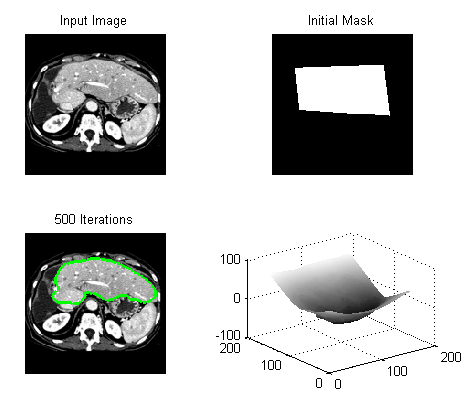
\includegraphics[scale=0.6]{images/matlab.png}
	\caption{MATLAB user interface showing four subfigures with the input image, the initial mask, the current zero level set interface superimposed on the input image and the current level set surface in 3D}
	\label{fig:matlab}
\end{figure}

The level set function $\phi$ is then initialised to a signed distance function of this mask, and iteration of the level set equation begins for a fixed number of iterations (also user-definable). Reinitialisation of the level set is performed once every 50 iterations, and the current level set contour and surface are displayed every 20 iterations.

The derivatives are calculated by subtracting shifted matrices of $\phi$ from $\phi$ (or vice-versa). Note how derivatives are not calculated in an element by element fashion.

The MATLAB code also features the Courant-Friedreichs-Lewy (CFL) condition which was described in section \ref{stability} to enforce stability, instead of arbitrarily defining $\Delta t$.

Finally, the user has the option of downsampling the input image in order to speed up the computation.

The MATLAB code was later adapted to 3D volume segmentation.

	\subsection{C}
Initially C code was written to most closely mirror the MATLAB code. The C code would serve as check for the parallel implementations to ensure correct values were calculated, the \textit{gold} version. The feature image, level set function, and derivatives were stored in memory as one dimensional arrays. These arrays were stepped through by nested for loops, looping $i$ looping $j$. To go from the two dimensional $i,j$ indices to a one dimensional index \textit{ind}, the equation $\textrm{ind} = j \times \textrm{imageW} +i$ was used. These for loops computed the derivatives serially, as shown in the pseudocode for algorithm \ref{alg:forloop}. This approach favoured itself well to being optimized at a low level using pointers to quickly step through the data. It was inefficient from a memory management perspective, with the derivative arrays taking up large amounts of memory for large image sizes, and also continuously being allocated and freed at each iteration.

\begin{algorithm}[h]
\BlankLine
\dontprintsemicolon
\ForAll{$i,j$}{
Calculate $D_x$\;
}
\ForAll{$i,j$}{
Calculate $D_y$\;
}
\ForAll{$i,j$}{
Calculate $D_z$\;
}
\ForAll{$i,j$}{
Calculate $D_x^+$\;
}
\BlankLine
...\;
\BlankLine
Update Level Set Function $\phi(t+\Delta t) =\phi(t) + \Delta t F|\nabla\phi|$\;
\caption{Pseudocode for Version 1 of Sequential C Code}\label{alg:forloop}
\end{algorithm}

This C implementation did not feature the versatility of the MATLAB implementation as it only accepted bitmap images as the input for the feature image. The loader function for the bitmap images (\texttt{bmploader.cpp}) is from the NVIDIA CUDA SDK image processing examples. It also did not feature any image resizing functions, as the focus was on optimization of the code and not versatility of inputs.

Wheras the MATLAB code used shifts of the matrix $\phi$ to calculate derivatives, in C the level set function $\phi$ was being stepped through in an element by element fashion. Therefore many boundary conditions had to be placed in order to ensure that derivatives took the value zero at certain boundaries. For example the forward difference derivative $D_x^+ =u_{i+1,j}-u_{i,j}$ must equal zero when $i=\textrm{imageW}$ as there is no $u_{i+1,j}$ term. The complexity of this task increases in three dimensions as there are six boundaries instead of four boundaries to condition for.

Restructuring the code for parallel computation of derivatives (using only one for loop) laid the framework for parallelization in CUDA, and only had a minor impact on performance. In this case all the derivatives are calculated at the same time at a given pixel, as shown below in algorithm \ref{alg:forloop2}. Also, the derivatives no longer needed to be stored in memory as arrays, and were simply floating point variables declared at each iteration. These two changes condensed the C code greatly.


\begin{algorithm}[h]
\BlankLine
\dontprintsemicolon
\ForAll{$i,j$}{
Calculate $D_x$\;
Calculate $D_y$\;
Calculate $D_z$\;
Calculate $D_x^+$\;
\BlankLine
...\;
}
\BlankLine
Update Level Set Function $\phi(t+\Delta t) =\phi(t) + \Delta t F|\nabla\phi|$\;
\caption{Pseudocode for Version 2 of Sequential C Code}\label{alg:forloop2}
\end{algorithm}

For the distance transform initialization and reinitialization procedures a seperate function was called. This is the \texttt{sedt2d} (Signed Euclidean Distance Transform in 2D) function written by Timothy Terriberry.

In order to visualise the level set evolution the combination of OpenGL and GLUT (OpenGL Utility Toolkit) was used to render the current zero level set. Rendering code was kept as compact and efficient as possible in order to have as minimal an effect as possible on performance whilst also making the program more comparable with the MATLAB code. Its principal purpose was of course to visualise how the level set was evolving (checking for instabilities, incorrect parameters for thresholding, range and curvature) and view the final segmentation. 

\section{Parallel Implemention}
	\subsection{Unoptimized Version}
The first parallel implementation followed the structure shown in the pseudocode below. In CUDA, it is assumed that both the host and device maintain their own DRAM \cite{cuda}. Host memory is allocated as before using \texttt{malloc} and device memory is allocated using \texttt{cudaMalloc}. As memory bandwidth between the host memory and device memory is low (it is much lower than the bandwidth between the device and the device memory), it is recommended to keep the number of transfers to a minimum. In order to minimise the latency of accessing the shared memory it is recommended to make the block size a multiple of 16 and use the \texttt{cudaMallocPitch} routine to allocate memory with padding if the array's $x$ dimension is not a multiple of 16. Therefore most CUDA programs follow a standard structure of initialization, host to device data transfer, compute, and finally memory transfer of compute results from device to host. 

Unfortunately the algorithm for computing signed distance transforms is not executed in CUDA and creating one from scratch would have been beyond the scope of this project. Therefore device to host memory transfers were required every time reinitialization was necessary. Of course, when timing it is possible to stop and start timers during this process.

	
\begin{algorithm}[h]
\dontprintsemicolon
\BlankLine
\SetLine
Initialise $\phi_{i,j}^(0), D$ on host memory\;
Allocate memory for $\phi_n ,\phi_{n+1}, D$ on device\;
Copy $\phi_0 , D$ from host to device\;
\ForAll{$N$ Iterations}{
Execute Level Set Update CUDA Kernel $\phi_{i,j}^(n+1) =\phi_{i,j}^(n) + \Delta t F|\nabla\phi_n|$\;
Swap pointers of $\phi_{i,j}^(n) ,\phi_{i,j}^(n+1)$\;
\If{Iterations \% 50 == 0}{
Copy $\phi$ from device to host\;
Reinitialise $\phi$ to S.D.F\;
Copy $\phi$ from host to device\;
}
}
Copy $\phi$ from device to host\;
\caption{Parallel Implementation Pseudocode}\label{alg:cuda1}
\end{algorithm}	

CUDA threads are assigned a unique thread ID that identifies its location within the threadblock and grid. This provides a natural way to invoke computation across the image and level set domain, by using the thread IDs for addressing.  This is best explained with the tables below. Assume our image has dimensions $4\times 4$ and the block size is $2 \times 2$. Invoking the kernel with a grid size of $2 \times 2$ results in the 16 threads shown in table \ref{table:threads}, in the form (\texttt{threadIdx.y},\texttt{threadIdx.x}). These threads are grouped into blocks of four, as shown in table \ref{table:blocks}, in the form (\texttt{blockIdx.y},\texttt{blockIdx.x}). 

\begin{table}
\begin{center}
  \begin{tabular}{ | c | c || c | c |}
    \hline
    (0,0) & (0,1) & (0,1) & (0,1) \\ \hline
    (1,0) & (1,1) & (1,0) & (1,1) \\ \hline\hline
    (0,0) & (0,1) & (0,0) & (0,1) \\ \hline
    (1,0) & (1,1) & (1,0) & (1,1) \\
    \hline
  \end{tabular}
\end{center}
\label{table:threads}\caption{Thread IDs of 16 threads grouped into 4 blocks}
\end{table}

\begin{table}
\begin{center}
  \begin{tabular}{ | c | c |}
    \hline
    (0,0) & (0,1)  \\ \hline
    (1,0) & (1,1)  \\ \hline
  \end{tabular}
\end{center}
\label{table:blocks}\caption{Block IDs of 4 blocks grouped into a grid}
\end{table}

As each thread has access to its own \texttt{threadIdx} and \texttt{blockIdx} global indices ($i,j$) can be determined using the equations

\begin{verbatim}
           int i = blockIdx.x * blockDim.x + threadIdx.x;
           int j = blockIdx.y * blockDim.y + threadIdx.y;
\end{verbatim}

where \texttt{blockDim.x} and \texttt{blockDim.y} represent the dimensions of the block (which in this case are both equal to 2). It should be noted that the size of these block sizes affect kernel performance greatly and that much larger block sizes are used (in the proceeding algorthms typical block sizes are $32\times 4$ or $16 \times 8$). The effect of different block sizes on performance is analysed in Section \ref{results}.

Once these indices were set up, only minor tweaks were needed until the code was performing well. Although this code exhibited speedups over the single threaded implementation, there was still significant optimization to perform as a great deal of computation time was being wasted on access global memory continuously. Therefore this is a \textit{naive} implementation.

Some features such as the CFL condition, could not be implemented in this parallel version without slowing down computation time significantly. This is because such a condition requires the determination of the largest element of $\nabla\phi$ which is computed roughly half way through the update procedure. Therefore integrating this condition would require transferring $\nabla\phi$ and curvature terms back to host memory to determine $max\left\{F|\nabla\phi|\right\}$. The cost of this added complexity and slowdown outweighed the benefits, and therefore $\Delta t$ was chosen to be a free parameter.





	\subsection{2D Shared Memory Optimization}
In order to keep the number of costly accesses to device memory at a minimum, effective use of the on-chip shared memory is essential. This along with maximizing parallel execution and optimization of instruction usage form the three main performance optimization strategies for CUDA \cite{cuda}.

Integrating use of the shared memory into the CUDA kernel requires partitioning the level set domain into tiles. For first order finite difference problems such as this each tile must also contain values for neighbourhood nodes (often known as \textit{halo} nodes) for the $i\pm1$ and $j\pm1$ elements, so these must also be read into shared memory. As the size of the shared memory is only 16 KB, the sizes of the tiles and corresponding halo are limited. \cite{3dfinitedifference} outlines a framework for such a process that may serve as a good model for a multi GPU implementation, however the kernel will need to be modified as it is optimized for higher order stencils (without cross-derivative terms). Instead, tiling code was adapted from Giles' (2008) 'Jacobi iteration for Laplace discretisation' algorithm \cite{mgiles} which supports cross-derivatives well. The shared memory management technique in this finite difference algorithm accelerated the global memory implementation by over an order of magnitude.

The two dimensional segmentation algorithm does not require any $k\pm1$ terms, making the shared memory management more straightforward. For a block (and tile) size of $BX\times BY$ there are $2 \times (BX + BY +2)$ halo elements, as can be seen in Figure \ref{fig:shared2d}. In this figure the darker elements represent the thread block (the active tile) and the lighter elements represent the halo. It is in this manner that the domain of the computation is partitioned and this results in overlapping of the halo nodes.\\

\begin{figure}[h]
	\centering
		\includegraphics[scale=0.5]{images/shared2d.PNG}
	\caption{2D Shared Memory Arrangement}
	\label{fig:shared2d}
\end{figure}


Each thread loads  $\phi_n$ values from global memory to the active tile stored in shared memory. However, depending on the location of the thread within the thread block it may also load a single halo node into the shared memory. Therefore in order to load all halo nodes, this technique assumes that there are at least as many interior nodes as there are halo nodes. Before data can be loaded into the halos, the thread ID needs to be mapped to the location of a halo node both within the halo and within the global indices. The segment of code that sets up the halo indices (both local and global) for loading into shared memory is shown below, code is from \cite{mgiles}.

\begin{spacing}{1.1}
\begin{verbatim}
k    = threadIdx.x + threadIdx.y*BLOCK_X;
  halo = k < 2*(BLOCK_X+BLOCK_Y+2);

  if (halo) {
    if (threadIdx.y<2) {               // y-halos (coalesced)
      i = threadIdx.x;
      j = threadIdx.y*(BLOCK_Y+1) - 1;
    }
    else {                             // x-halos (not coalesced)
      i = (k%2)*(BLOCK_X+1) - 1;
      j =  k/2 - BLOCK_X - 1;
    }
\end{verbatim}
\end{spacing}

The first $2 \times (BX + BY +2)$ threads are assigned to load values into the halo in this manner. This is best visualised with the example of a $6 \times 6$ thread block as shown below in Figure \ref{fig:haloloading}.

\begin{figure}[h]
	\centering
		\includegraphics{images/halo.pdf}
	\caption{Tile and halo showing for a $6 \times 6$ block the mapping of thread IDs to halo nodes}
	\label{fig:haloloading}
\end{figure}


This method of loading elements has been chosen in order to maximise \textit{coalescence}. Not only are the interior tile nodes loaded coalesced, but as can be seen above, the first 12 elements of the thread block load the $y$ halos (above and below the the interior tile excluding corners) in a coalesced manner. The side halos ($x$ halos) loads are non-coalesced. When writing back results to global memory, as only the interior nodes have updated values they are written to global memory coalesced.

\subsection{3D Shared Memory Optimization}


In three dimensions, $k\pm1$ terms are required and therefore these values need to also be stored in shared memory. CUDA only allows for two dimensional grid sizes (even though blocks can be three dimensional), implying that the number of blocks in the $z$ dimension cannot exceed 1.
 
\begin{figure}[h]
	\centering
		\includegraphics[scale=0.5]{images/shared3d.PNG}
	\caption{3D Shared Memory Arrangement}
	\label{fig:shared3d}
\end{figure}

The algorithm by Giles \cite{mgiles} uses three $k$-planes of data for this purpose as shown in Figure \ref{fig:shared3d}.



Before looping over the $k$-planes begins, the $\phi_k$ plane is loaded into the $k+1$ plane of shared memory. Upon entering the loop this plane is shifted down one plane to the $k$ plane and the $\phi_{k+1}^n$ plane is loaded into the $k+1$ plane. Level set function values for $\phi_{k}^{n+1}$ are calculated and written coalesced back to global memory. The $k$ plane is then shifted to the $k-1$ plane, the $k+1$ plane is shifted to the $k$ plane, and new values are loaded from $\phi_{k+1}^n$ to the $k+1$ plane. This looping over the $z$ dimension continues for all $z<\textrm{imageD}$. In this manner, each block actually processes a $BX \times BY \times \textrm{imageD}$ sub domain.

